\documentclass[10pt,a4paper]{article}
\usepackage[margin=1in]{geometry}
\usepackage[utf8]{inputenc}
\usepackage{amsmath}
\usepackage{amsfonts}
\usepackage{amssymb}
\usepackage{natbib}
\bibliographystyle{plainnat}
\usepackage{hyperref}
\usepackage{graphicx}
\usepackage{multirow}
\usepackage{subcaption}
\usepackage{array}
\usepackage{booktabs}
\graphicspath{figs/}
\renewcommand{\arraystretch}{1.2}
\renewcommand{\d}{\mathrm{d}}

\author{Claire Marie Guimond \\ Dr. Oliver Shorttle \& Dr. John Rudge, supervisors \\ First-Year Report to the Department of Earth Sciences of the University of Cambridge}
\title{Mountains on massive rocky exoplanets?: \\ \Large Theoretical limits to topography}


\begin{document}

\maketitle

\section*{Abstract}

Topography is a crucial component of the Earth system: having exposed fresh rock lets surface temperatures self-regulate via silicate weathering. However, there are limits to a lithosphere’s capacity to support mountains or valleys over geologic time. We see in our solar system that the range in a body’s elevations tends to decrease with increasing planet mass. Meanwhile, most currently-known exoplanets are in between the sizes of Earth and Neptune---a regime totally exotic to the solar system---and many have apparent bulk densities consistent with a rocky composition. Our aim is to extrapolate solar system trends in topography to massive rocky exoplanets using well-studied geodynamics models. This builds on current work in understanding the limits of terrestrial planet thermal evolution models. Given these models, we can predict the range of dynamically-supported, and eventually, elastically-supported topography. Specifically, we are after how massive an exoplanet can be before it becomes hypsometrically featureless.

\tableofcontents
\listoffigures

\section{Background}

The interior of a planet affects its surface character. Motions in the mantle are continuously modulating important aspects of the entire planetary system like the volume of its oceans, the composition and pressure of its atmosphere, its surface elasticity, its magnetic field, and its overall climate and habitability \citep{Noack2014, Foley2016, Wordsworth2016, Tosi2017, Wordsworth2018, Shahar2019}. This fact is not always explicit in studies of exoplanets \citep{Shahar2019}, as astrophysics cannot directly constrain geophysical models. Nevertheless, advances brought on by the characterization era of exoplanet science\footnote{i.e., atmospheric spectroscopy} now permit some description of planetary interiors as well, through measurements of a planet's bulk density, the host star chemistry, and the detection of atmospheric species \citep{Santos2017, Dorn2017, Dorn2017a, Dorn2018, Bower2019, Madhusudhan2020}. In this way, exoplanet science is an intrinsically interdisciplinary field, drawing on geophysics and geochemistry to study planets around other stars.

Not only can Earth teach us about exoplanets, but exoplanets can place Earth in an illuminating context. We now know exoplanets are as common as stars, so even basic measurements across a sample have statistical power to complement more detailed studies of the cosmically-unrepresentative solar system. Indeed, other planetary systems are found to be very unlike the one we know: the first detection of an exoplanet revealed this fact with a bafflingly close-in Jupiter-mass world \citep{Mayor1995}. As exoplanet occurrence rate studies reveal \citep{Petigura2013, Foreman-Mackey2014, Dressing2015, Kunimoto2020}, every Sun-like star\footnote{FGK spectral class} in the solar neighbourhood is statistically likely to host at least one planet of mysteriously intermediate mass, between Earth and Neptune---before the detection of exoplanets we had no reason to imagine these existed. 

In the interim, before more detailed observational constraints on massive potentially-rocky planets can be made, there grows a theoretical literature on how geophysical matters scale with mass: internal structure \citep{Valencia2006, Zeng2017}, tidal response \citep{Tobie2019}, outgassing \citep{Kite2009, Noack2017, Dorn2018a}, geodynamos \citep{Gaidos2010}, tectonics \citep{ONeill2007, Korenaga2010}, and so on. Here we are interested in the planet mass-scaling of a particular expression of interior dynamics not typically considered in the exoplanet context: the occurence of topography. Topography is tightly linked to temperatures and mantle flows inside the planet. Therefore the problem is one of understanding a planet's thermal history.

\subsection{Terrestrial planet interiors through time}

%The late stage of planetary accretion leaves a molten and unrecognizable world \citep{Elkins-Tanton2012}. The magma ocean planet crystallizes to rock \footnote{unless the planet's surface is kept too hot such as by proximity to the star, in which case crystallization can take 100 million years, not a few million \citep{Hamano2013}.}, and during cooling, the interior gravititationally differentiates, and volatile species partition between the mantle and the primary crust and atmosphere. These processes set the ``intitial" thermal and chemical state of the solid planet \citep{Tosi2019}. 

The transport of heat through a planet drives much of its dynamics. In the broadest sense, the thermal state of the planet can be described by the ratio of heat production to heat loss; that is, the Urey ratio:
\begin{align}\label{eq:Ur}
{\rm Ur} = \frac{Q_{\rm radiogenic}}{Q_{\rm surface}},
\end{align}
where $Q_{\rm radiogenic}$ and $Q_{\rm surface}$ are the whole planet-integrated fluxes in W of radiogenic heating and surface heat loss, respectively. A young planet can have so much radiogenic heating power that its Ur is much larger than 1.\footnote{For example, from $^{26}$Al, which drives differentiation.} Three things happen to a planet with age: the hot core transfers its excess heat into the mantle; its interior abundances of potassium-40, uranium-235, uranium-238 and thorium-232 decline; and the surface loses heat to the atmosphere and eventually to space. This thermal evolution is described via the energy balances,
\begin{align}\label{eq:T_ODE}
\begin{split}
M_m c_{m} \frac{{\rm d}T_m}{{\rm d}t} &= -Q_{\rm u} + Q_{\rm rad} + Q_c, \\
M_c c_{c} \frac{{\rm d}T_c}{{\rm d}t} &= -Q_c,
\end{split}
\end{align}
where $M_m$ is the mantle mass in kg, $c_{m}$ is the mantle specific heat capacity in J kg$^{-1}$ K$^{-1}$, $Q_{\rm rad}$ is the mass-integrated radiogenic heat flux in W, $Q_{u}$ is the magnitude of the surface-integrated heat flux out of the top of the mantle in W (the subscript $u$ denotes the upper boundary layer). The analagous notation with subscript $c$ applies to the core. Although (\ref{eq:T_ODE}) oversimplifies the problem by omitting other heat fluxes like volcanism, it will suffice in capturing the basic behaviour \citep{Jaupart2015}.



\subsection{Parameterized convection models}

The temperature difference between the core-mantle boundary and the lithosphere drives convection, a process that has been modelled to varying degrees of complexity \citep[e.g.,][]{McKenzie1974, Nakagawa2015}. While 3D models include more subtleties than lower-dimensional models, running them is computationally expensive. Cheaper 1D parameterized convection models are more reasonable for certain reasearch questions \citep{Sharpe1979, Schubert1980, Davies1980}. When investigating distant planets' topography, where we have little-to-no constraints on the model parameters, computational inexpensiveness allows us to explore a much larger parameter space. Conversely, numerical convection models are better used to predict, for example, the exact shape and distribution of surface topography on Earth or Venus \citep[e.g.,][]{Moresi1995, Vezolainen2004}. 1D parameterized models have previously been applied to planets larger than Earth \citep{Valencia2009, Stamenkovic2012}.

Parameterized models can be successful in capturing convection's effect on planetary heat budgets because most of the key behaviour of a convecting cell is controlled by relatively thin thermal boundary layers at the top and bottom of the cell---boundary layers are where the cell's thermal history is effectively determined. Parameterized models will be therefore be valid as long as dynamic processes in the thermal boundary layers occur faster than the planet loses heat \citep{Sharpe1979, Korenaga2008a}. 

As detailed in the appendix to this report, one can write scaling laws for the heat fluxes across the thermal boundary layers. The heat fluxes ultimately depend on the Rayleigh number, Ra. Ra is a nondimensional parameter which quantifies the ``vigour" of convection, and is equal to the ratio of time scales for heat transport by conduction to heat transport by convection:
\begin{equation}\label{eq:Ra}
\mathrm{Ra} = \frac{\tau_{\rm conduction}}{\tau_{\rm convection}}= \frac{\alpha \rho g \Delta T d^3 }{ \kappa \eta(T)},
\end{equation}
where $\alpha$ is thermal expansivity in K$^{-1}$, $\rho$ is density in kg m$^{-3}$, $g$ is surface gravity in m s$^{-2}$, $\Delta T$ is the temperature contrast across the layer in K, $d$ is the thickness of the layer in m, $\kappa$ is the thermal diffusivity in m$^{2}$ s$^{-1}$, and $\eta$ is the dynamic viscosity in Pa s. For a non-isoviscous convecting cell in 2D or 3D, there are many values of viscosity to choose from when defining Ra, so the location this viscosity corresponds to must be specified. Different types of Rayleigh numbers exist, which make different assumptions about what quantity is fixed in the model (the ``thermal" Ra in (\ref{eq:Ra}) fixes $\Delta T$), so we must be cautious when comparing between them.

Below a critical Rayleigh number, Ra$_{\rm crit}$, convection is so weak it halts altogether. The value of Ra$_{\rm crit}$ depends on the wavelength of the disturbance that initiates convection, but often a constant value is assumed for a planetary mantle. The Ra number controls the thermal boundary layer in that the thickness of this layer, $\delta_u$, is approximately the value of $d$ at which convection is inefficient, Ra = Ra$_{\rm crit}$ locally. Therefore $\delta_u \propto {\rm Ra}^{-3}$.

The flux across the upper thermal boundary layer, $q_u$, scales with Ra via $\delta_u$:
\begin{equation}\label{eq:q_Ra}
q_{u} = -k_m \frac{a_{rh} \Delta T_{rh}}{\delta_{u}},
\end{equation}
where $k_m$ is the thermal conductivity in W m$^{-1}$ K$^{-1}$, $\Delta T_{rh}$ is the rheological temperature scale in K, set by the rate of change of viscosity with temperature (see Appendix \ref{sec:methods}), $a_{rh}$ is a constant of order unity, and $q_u$ is in W m$^{-2}$.




\subsection{Regimes of mantle convection}

Stagnant lids appear to be a natural consequence of temperature-dependent convection. Laboratory experiments observing cells of convecting corn syrup or golden syrup show that if the viscosity contrast between the centre and surface is large enough, the upper part of the thermal boundary layer will be dynamically-decoupled from the interior; i.e., not participate in convection at all. These so-called stagnant lids develop in convection cells with large viscosity contrasts \citep{Davaille1993, Giannandrea1993}. Silicate rock has a strongly temperature-dependent rheology \citep{Karato1993}, and indeed Venus and Mars seem to behave as if they have a stagnant lid. Heat flows through the lid via conduction, while convection occurs only below the lid, where conditions are hotter and more viscous \citep{Morris1984, Christensen1984, Hansen1993, Solomatov1995}. %This fact inspires many questions about whether stagnant lid planets can form ``continents" and other topographic complexities. The character of certain tesserae on Venus imply tectonic origin, questioning whether this world always had a purely stagnant lid \citep{Bindschadler1991, Lenardic1991}. 
This scenario is illustrated in figure \ref{fig:stagnant_lid}.

Stagnant lid behaviour has been reproduced numerically \citep{Solomatov1995, Moresi1995a, Solomatov1996a}. Maps of convective regimes in viscosity contrast-Rayleigh number space can be found in \citet{Solomatov1996a} and more recently in \citet{Huttig2011} and \citet{Miyagoshi2015}, with stagnant lids favouring higher Rayleigh numbers \textgreater~$10^{6}$--10$^{7}$ and viscosity contrasts \textgreater~$10^4$ between the interior mantle and the surface.

We consider a stagnant lid regime under the premise that it represents a ``default" rocky planet \citep{ORourke2012}. In our own solar system, rocky planets are more frequently found in a stagnant lid regime than in a plate tectonic regime. With the assumption of a stagnant lid we avoid some unknown complexities that mobile plates introduce. Namely, plate margin-dominated heat loss on Earth works differently \citep[and more efficiently---stagnant lid planets will run hotter for the same rheology and surface heat flow;][]{Stevenson2003} than in a stagnant lid regime, where heat loss is simply determined by boundary layer scaling laws like those we have discussed.


\begin{figure}

  \centering
  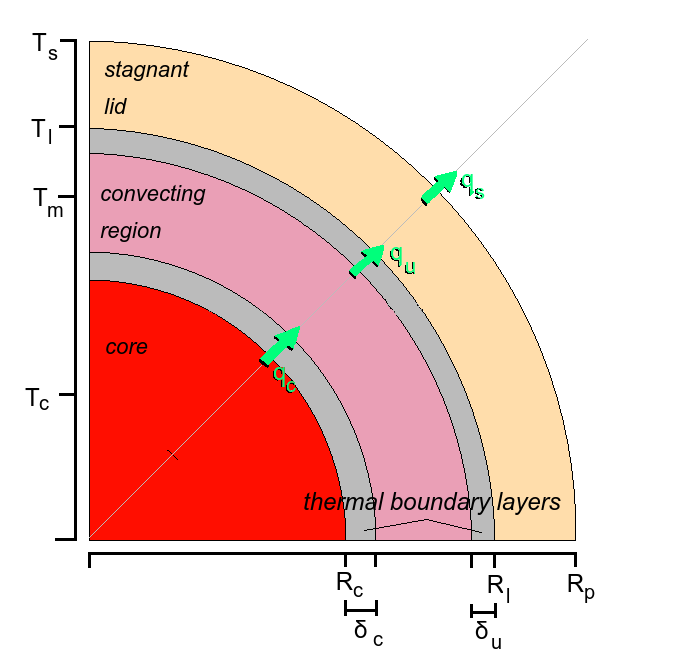
\includegraphics[width=0.5\linewidth]{stagnantlid}

\caption{Structural model of a stagnant lid planet, not to scale. $R_p$ is the radius of the planet, $R_l$ is the radius at the base of the lid, $R_c$ is the radius of the core, $T_s$ is the surface temperature, $T_l$ is the temperature at $R_l$, $T_m$ is the isothermal convecting cell temperature, $T_c$ is the isothermal core temperature, and $\delta_u$ and $\delta_c$ are the upper and lower thermal boundary layer thicknesses respectively. The boundary layer heat fluxes $q_c$ and $q_u$ and the surface heat flux $q_s$ are defined in equations (\ref{eq:q_Ra}) and (\ref{eq:q_s}), respectively}. 
\label{fig:stagnant_lid}
\end{figure}







\subsection{Stress and topography}

Earth is hypsometrically bimodal: continents and oceans form separate peaks in the hypsometric curve. This is a complexity not seen on Mercury, Venus, the Moon, or Titan \citep{Keller2009, Lorenz2011}.\footnote{Mars has dichotomous crustal thickness split between its north and south hemispheres. This produces bimodality for different reasons than Earth, a further complexity.} Earth's topography is much more convoluted than anything a parameterized convection model could predict. Topography on stagnant lid planets, however, is more tenable to modelling.


\subsubsection{Mechanisms of topographic support}\label{sec:top_mechs}


To predict topography, we need to look at the forces balancing topographic loads. The first two mechanisms we discuss are not the focus of this document, but are nevertheless associated with the most dramatic topography on planets:
\begin{enumerate}
\item \emph{Elastic flexure} of a shell supports loads by way of elastic stresses that develop in the lithosphere;
\item \emph{Compositional isostasy} occurs when high mountains made of low-density crust are underlain by either deep roots of the same low density (Airy model), or by roots of the same thickness as the surrounding plain but of lower density (Pratt model).
\end{enumerate}
Whether a load is supported by (1) or (2) is set by the ratio of the width of the load to a flexural parameter, which depends on the lithosphere's elastic properties.\footnote{$\alpha_{\rm flex} = \left[\frac{1}{3(1 - \nu^2)}\frac{Ed_e^3}{\rho_m g}\right]^{1/4}$, where $d_e$ is the lithosphere thickness, $\rho_m$ is the underlying mantle density, $\nu$ is Poisson's ratio, and $E$ is Young's modulus.}
%\begin{equation}
%\alpha_{\rm flex} = \left[\frac{1}{3(1 - \nu^2)}\frac{Ed_e^3}{\rho_m g}\right]^{1/4},
%\end{equation}
%where $d_e$ is the lithosphere thickness, $\rho_m$ is the underlying mantle density, $\nu$ is Poisson's ratio, and $E$ is Young's modulus. 
If the width of a load is smaller than the flexural parameter, elastic stress in the lithosphere will support the load. If the width is much larger, buoyancy forces will support it. Hence flexure is associated with short-wavelength topography and isostasy is associated with long-wavelength topography. 

The last support mechanism is borne by convection in the interior. Historically the term has always not referred to the same phenomena, so it is helpful to break down \emph{dynamic topography} further \citep{Orth2011, Molnar2015} into:
\begin{enumerate}
\setcounter{enumi}{2}
\item \emph{Flow-induced tractions} on the base of the lithosphere. These tractions are exerted by the deformation of density boundaries within the viscously-flowing material below the thermal boundary layer.
\item \emph{Thermal isostasy,} variations in the thickness and thermal structure of the upper boundary layer \citep{Fowler1985}. On Earth this can be split into lithospheric and aesthenospheric components, but for planets without plates, this collapses to just variations in the viscous lid \citep[see][]{Orth2011}. This is unlike Airy and Pratt isostasy in that the density contrasts are thermal rather than compositional. Thermal isostasy provides the majority of ``dynamic topography."\footnote{Analytically we expect component 4 to dominate component 3 for an idealized sine-curve temperature perturbation at the surface, regardless of the wavelength of that perturbation \citep{McKenzie1977}. It can be shown that the gravity anomaly $\Delta g_1(x)$ considering no density contrast in the lithosphere, just the lithosphere's deflection upwards, is $\Delta g_1(x) = 2\pi G \Delta \rho \Delta h(x)$, where $G$ is the gravitational constant and $\Delta h$ is the height of topography. The gravity anomaly $\Delta g_2(x)$ associated with the flow-induced density contrasts alone is $\Delta g_2(x) = 2\pi/3 \; G\rho\Delta h_2(x)$. For a given gravity anomaly, $\Delta h_1 > \Delta h_2/3$.}
\end{enumerate}
Together, components 3 and 4 make the ``full dynamic topography."
%The distinction between components 3 and 4 matters, not necessarily because different parties disagree with their competing importance (on Earth), but because ``dynamic topography" does not consistently refer to either or both components. %In some circumstances, the two mechanisms can even produce identical signals \citep{Molnar2015}. 



%It can be shown that the topography associated with (3) is about a third of the topography associated with (4) \citep{McKenzie1968, McKenzie1977, Molnar2015}. 


\subsubsection{Dynamic topography forward models}\label{sec:dyn_top_forward}

%\citet{McKenzie1968, 1977} derives analytic half-space equations for $\Delta h$ as a function of a harmonic temperature perturbation $T(x) = T_0 \cos(2\pi x/\lambda)$, associated with both static and dynamic density contrasts, In both cases the solution for $\Delta h(x)$ is propotional to $\alpha T_0 \lambda / (2\pi) \cos(2\pi x/\lambda)$, with the static scenario a factor of \nicefrac{4}{3} higher because it does not have to overcome resistance to flow from an additional vertical shear stress term (Stokes equation). 

Numerical models can calculate the amplitude of the dynamic component of topography, $\Delta h$, by solving the equations of motion and the heat transport equation for a convecting cell, and obtaining the velocity and temperature fields. The total stress in the vertical direction, $\tau_{zz}$, can then be calculated at the surface of the cell. Total vertical stress is given by 
\begin{equation}\label{eq:tau_zz}
\tau_{zz} = 2\eta \; \frac{\partial u_z}{\partial z} - p_1,
\end{equation}
where $\partial u_z / \partial z$ is the vertical velocity in m s$^{-1}$ and $p_1$ is the pressure pressure perturbation from thermal convection in Pa \citep{Parsons1983}. The first term in (\ref{eq:tau_zz}) is the viscous stress. The hydrostatic pressure $p_0$ of a topographic load balances this stress, $p_0 = \rho g \Delta h = \tau_{zz}$, where $\Delta h$ is in m. Combining this and (\ref{eq:tau_zz}) with self-consistent pressure and temperature profiles inherently includes both dynamic topography components, producing the full dynamic topography,
\begin{equation}\label{eq:h_stress}
\Delta h = \frac{\tau_{zz}}{\rho g}.
\end{equation} 




In principle, one can obtain $\tau_{zz}$ in (\ref{eq:tau_zz}--\ref{eq:h_stress}) from parameterized convection, since the upper thermal boundary layer contributes most of the depth-integrated stress \citep{Parsons1983, Solomatov1995}. The parameterized stress is given by
\begin{equation}\label{eq:tau_param}
\tau_{zz} = C_1 \rho_m g_{\rm sfc} \alpha_m \Delta T_{rh} \delta_u.
\end{equation}
\citet{Reese2005} give proportionality constant $C_1 = 2$ for the shear stress at the lid generated by sinking plumes, based on fits to a numerical convection model with spherical geometry and temperature-dependent viscosity. We note that it is the normal component of stress, not the shear stress, that balances $\rho g \Delta h$. %However, no other scaling is available to our knowledge, so we adopt this value as a preliminary measure.

If we treat $\tau_{zz}$ as the planetary root-mean-square (RMS) value for convective stress, then we can use (\ref{eq:tau_param}) to produce the RMS dynamic topography, $\Delta h_{\rm RMS}$. This is distinct from the peak altitude $\Delta h_{\rm peak}$ of a given dynamically-supported topographic feature (that is, the maximum height of the surface topography over an individual mantle plume). Conversion between $\Delta h_{\rm RMS}$ and $\Delta h_{\rm peak}$ is not simple, as we will see in section \ref{sec:results-comparison}. Nevertheless, different studies are concerned with calculating either one or the other, and we omit neither type of study.

According to (\ref{eq:tau_param}), we expect $\Delta h_{\rm RMS}$ to reflect the RMS thermal boundary layer thickness, which we take to be equivalent to the instantaneous value of $\delta_u$ in a 1D model. Again, this scales with Ra as $\delta_u \propto {\rm Ra}^{-3}$. The strength of this scaling would be affected by other modelling decisions, such as the geometry, the rheology law, and the amount of internal heating compared to basal heating \citep{McKenzie1977}. Under particular model assumptions, scalings of $\Delta h$ with Ra can be found in the existing literature.

For the first and most basic scaling, we combine (\ref{eq:h_stress}) and (\ref{eq:tau_param}) in terms of Ra via (\ref{eq:d_u}):
\begin{equation}\label{eq:dyn_top_stress}
\Delta h_{\rm RMS} \sim \alpha_m d \Delta T_{rh} \left(\frac{\rm Ra}{\rm Ra_{\rm crit}}\right)^{-\frac{1}{3}}.
\end{equation}
(\ref{eq:dyn_top_stress}) is equivalent to equation (34) in \citet{Parsons1983}, which is a boundary-layer-based approximation of their equation (33),
\begin{equation}\label{eq:PD83_0}
\Delta h = C_2 \frac{\eta_m \kappa_m}{\rho_m g d^2} \left({\rm Ra}_F\right)^n,
\end{equation}
where Ra$_F$ is the Rayleigh number based on surface heat flux,\footnote{Ra$_F = (\rho g \alpha d^4 q_u)/(k \kappa \eta)$} $n = 0.5$ \citep{McKenzie1977}, and $C_2 = 5.4$ to match the predictions of RMS dynamic topography in \citet{Lees2019} using a 3D isoviscous basal-heating convection model. This value for $n = 0.5$ comes from boundary layer theory and represents the case where the boundary layer thickness is independent of the layer depth \citep{McKenzie1974}. The positive value of $n$ implies that topography increases with Ra$_F$ in this isoviscous scaling---this is misleading because there is a factor of $\eta$ outside of the exponential term, so for non-isoviscous situations, $ \Delta h \propto \eta^{4/3}$. If Ra is increased by decreasing $\eta$, then $\Delta h$ also decreases \citep{Nimmo1996}.


Although it can be misleading to convert between Ra and Ra$_F$ as the model assumptions are fundamentally different, we can approximate (\ref{eq:PD83_0}) as a function of Ra with $n = 0.5$, using Ra$^{4/3} = \Delta T_m / \Delta T_{rh} {\rm Ra}_{\rm crit}^{1/3} {\rm Ra}_F$. Making this approximate conversion results in an exponent on Ra of -1/3 in (\ref{eq:PD83_0}), equivalent to (\ref{eq:dyn_top_stress}). 





A second scaling is a direct log-log fit by \citep{Kiefer1992} to the \emph{peak} value of $\Delta h$ over a mantle plume versus Ra, using a 2D cylindrical isoviscous numerical convection model which they apply to Venus:
\begin{equation}\label{eq:KH92}
0.7 \Delta h = 66 {\rm Ra}^{-0.121},
\end{equation}
where the factor of 0.7 = $(\rho_m - \rho_{\rm ocean} / \rho_m)$ scales their water-loaded model to subaerial topography. We further scale this $\Delta h$ by 0.707 (the RMS value of a sine wave) to approximate $\Delta h_{\rm RMS}$.

 



If one wishes to separate the thermal and flow-induced components of (\ref{eq:tau_zz}), expressions can be derived for the maximum topography due solely to thermal isostasy from thinning of the lithosphere: 
\begin{equation}\label{eq:h_th}
\Delta h \sim 0.5\alpha (T_i - T_s) z_{l, 0},
\end{equation}
where $T_s$ is the surface temperature in K, $T_i$ is the temperature below the lithosphere in K at the point of interest, and $z_{l, 0}$ is the average thickness of the lithosphere in m \citep{Kucinskas1994, Orth2011}. Because this thermal thinning component may explain most of the full dynamic topography on stagnant lid planets, (\ref{eq:h_th}) can be used instead of (\ref{eq:dyn_top_stress}) to approximate dynamic topography, if one knows how interior temperatures vary laterally \citep[the ``isostatic stagnant lid approximation";][]{Orth2011}. However, the fact that (\ref{eq:h_th} requires this 2D information precludes the isostatic stagnant lid approximation from being used with 1D convection models.























\begin{landscape}
\thispagestyle{empty}
%\begin{table}

\footnotesize


\begin{longtable}{ @{} p{4cm} r r p{2cm} p{2cm} r p{1.5cm} p{5cm} @{} } 
\caption{Predictions from numerical convection of dynamic topgraphies on Venus, with important model parameters noted. Internal heating is calculated as $(q_s - q_b)/q_s$, where $q_s$ and $q_b$ are the surface and basal heat fluxes in W m$^{-2}$ respectively. Reported values of the Rayleigh number are distringuished between that defined with a fixed temperature contrast, Ra (\ref{eq:Ra}), and that defined with a fixed basal heat flux, Ra$_B$. \;\;  *Calculated from the spherical harmonic power spectrum using $\Sigma_l [S(l)/(2l + 1)]^{1/2}$.} \label{tab:dyn_topo_obvs}\\

\toprule

\textsc{Reference} & \textsc{Peak} & \textsc{RMS} & \textsc{Location} & \textsc{Viscosity} & Ra & \textsc{Internal heating} & \textsc{Model type} \\
%\midrule

\; & \multicolumn{2}{c}{\textsc{Observed topography} (km)} \\
\cline{2-3} \\
%\textsc{Reference} & \textsc{Peak} & \textsc{RMS} & \textsc{Location}  \\
%\cline{1-4} \\


\citet{Smrekar1991} & \makecell[tr]{4.5 \\ 6.2 \\ 1.8} &  & \makecell[tl]{Beta Regio \\ Atla Regio \\ Asteria Regio} \\
\citet{Rappaport1999} &  &  0.96 &  \\


%\midrule
\; & \multicolumn{2}{c}{\textsc{Dynamic topography} (km)} \\
\cline{2-3} \\
%\textsc{Reference} & \textsc{Peak} & \textsc{RMS} & \textsc{Location} & \textsc{Viscosity} & Ra & \textsc{Internal heating} & \textsc{Model type} \\
%\midrule


\citet{Solomatov1996a} & \makecell[tl]{$\sim$4 \\ $\sim$2} & n/a  & \makecell[cl]{Beta Regio \\ Average} & $f(T)$  & Ra = $3 \times 10^7$  & 0\% & Cartesian 2D \\
%Beta Regio (avg) scaled so admittance is 30 (15) m/km, fixed $d_m$ = 1600 km 

\citet{Vezolainen2003} & 3.5--6 & n/a & Beta Regio & $f(T)$  & Ra = $3 \times 10^7$ & 0\% & Cartesian 2D   \\
%  fixed $\Delta T_m$ = 1100 K

\citet{Kiefer1991} & \makecell[tr]{7.5 \\ 5.2 \\ 3.6} & n/a  & Atla, Beta, Ovda, Thetis Regiones &  constant & \makecell[tr]{Ra = $10^5$ \\ Ra = $10^6$ \\ Ra = $10^7$} & 0\% & Cylindrical 2D   \\
% after  \citep{Hager1985}


%\citet{Kiefer1992} &  7.5  & n/a & Global & Ra = $10^6$ & $\eta_m$ constant with high-$\eta$ stagnant lid & Numerical cylindrical plume & (3) & for $D_{\rm lid}$ = 130 km; gives scaling laws with Ra, assumes no internal heating (bottom of page 203). h from figure 9 constant visc \\$f(T)$


\citet{Moresi1995} & \makecell[tr]{5.8 \\ 3.8 \\ 5.1} & n/a & Generic &  \makecell[tl]{$f(T)$ \\ $f(T,z)$ \\ $f(T,z)$} & \makecell[tr]{Ra$_B$ = 2.4 $\times 10^6$ \\ Ra$_B$ = 1.3 $\times 10^6$ \\ Ra$_B$ = 1.0 $\times 10^6$} & 0\% & Cylindrical 2D   \\
% Scaling: $\eta_0 \kappa / (d^2 \Delta\rho g)$ with $\eta_0$ from basal heating Ra, can't extrap to higher $\Delta\eta$ with linearized viscosity law. concerned with predicting admittance
 %

\citet{Nimmo1996} &  \makecell[tr]{1.16 \\ 1.47 \\ 2.85}  &  n/a  & Global & constant & \makecell[tr]{Ra$_B$ = 1.6 $\times 10^7$ \\  Ra$_B$ = 7.9 $\times 10^6$\\ Ra$_B$ = 4.0 $\times 10^6$ } & 0\% & Cylindrical 2D \\

\citet{Kiefer1998} &  5.4--10.9 & 1.6--2.7  & Global & constant & Ra = $10^6$ & 73 \% & Spherical axisymmetric 2D \\
% Scaling: $(\rho_m \alpha \Delta T R_p) / (\rho_m - \rho_s)$  internal heating Ra $10^7$






\citet{Vezolainen2004} & 5.7 & n/a & Beta Regio & $f(T)$  & Ra = $3 \times 10^7$ & 0\% & Cartesian 3D \\
%  fixed $\Delta T_m$ = 1100 K



%\citet{Orth2011} & 2.2 nondim & n/a  & Global &  Frank-Kamenetskii & Ra$_i$ = 10$^7$ & 0\% & 3D spherical shell & Thermal isostasy \\



\citet{Golle2012} & 3.3 & 2.7*  & Global & $f(z)$ & Ra$_b = 3.8\times 10^8$ & 0\% & Spherical 3D, viscoelastic  \\



\citet{Benesova2012} &  3.25 & n/a   & Alta Regio  & $f(z)$ & Ra = $2.8 \times 10^6$ & \textgreater 50\% & Spherical 3D  \\
% specifically say no thermal isostasy, although Orth thesis says they do implicitly?



\citet{Huang2013} & 2\textendash 3 & 0.75 & Global & $f(T,z)$ & Ra = $1.8\times 10^7$ & 75\% & Spherical 3D  \\
% goal is to simultaneously match number of plumes and GTR observations. semi-amplitude by eye from maps.  say case 15 is best fit to obvs. Ra fixed, using avg viscosity $2\times 10^{21}$ Pa s

\citet{Yang2016} & n/a & 0.27* & Global & $f(T,z)$ &  Ra = $7.3\times 10^6$ & 80\% & Spherical 3D \\
% they say "The gravity anomaly is the summation of that caused by the dynamic topography and by the density heterogeneity itself." and "the topography of volcanic rises is mainly due to dynamic uplift"


\bottomrule


\end{longtable}
%\end{table}
\end{landscape}


\begin{table}
\centering
\caption{Parameters used in this study. \label{tab:params}}
\footnotesize
\begin{tabular}{@{} c l r l p{4cm} @{}}
%\multicolumn{5}{l}{\textbf{Constant values for all planets}} \\
\toprule
Symbol & Description & Value & Units & Ref. \\
\midrule
\multicolumn{5}{c}{\textbf{Constant bulk properties}} \\
$\rho_c$ & Core density & 7200 & kg m$^{-3}$ &  \citet{Thiriet2019}  \\
$c_c$ & Core specific heat at constant volume & 840 & J kg$^{-1}$ K$^{-1}$  & \citet{Thiriet2019}  \\
$k_m$ & Mantle thermal conductivity & 4 & W m$^{-1}$ K$^{-1}$  & \citet{Thiriet2019}  \\
$\alpha_m$ & Thermal expansivity &  $2.5 \times 10^{-5}$ & K$^{-1}$  & \citet{Thiriet2019}  \\
$\kappa_m$ & Thermal diffusivity &  $1 \times 10^{-6}$ & m$^2$ s$^{-1}$  & \citet{Thiriet2019}  \\
$X_{\rm K}$ & Initial K abundance &  305 & wt ppm  & \citet{Jaupart2015} \\
$X_{\rm U}$ & Initial U abundance &  $16 \times 10^{-3}$ & wt ppm  & \citet{Jaupart2015} \\
$X_{\rm Th}$ & Initial Th abundance &  $56 \times 10^{-3}$ & wt ppm  & \citet{Jaupart2015} \\
$H_{4.5}$ & Radiogenic heating rate at 4.5 Gyr & $4.6\times 10^{-12}$ & W kg$^{-1}$ & \citet{Jaupart2015} \\
Ra$_{\rm crit}$ & Critical Rayleigh number & 450 &  & \citet{Thiriet2019}  \\
$E_a$ & Viscosity activation energy & 300 & kJ mol$^{-1}$ & \citet{Karato1993} \\
$A_{rh}$ & Viscosity preexponential factor & 8.7 $\times 10^{15}$ & & \citet{Karato1993} \\
$h_{rh}$ & Grain size & 2.07 & mm & \\
$B$ & Burgers vector & 0.5 & nm & \citet{Karato1993} \\
$m$ & Grain size exponent & 2.5 & & \citet{Karato1993} \\
$\mu$ & Shear modulus & 80 & GPa & \citet{Karato1993} \\
CMF & Core mass fraction & 0.3 & & \\
$L_*$ & Stellar luminosity & 1 & $L_{\rm Sun}$ &  \\
Al & Planetary geometric albedo & 0 & &  \\

\midrule
\multicolumn{5}{c}{\textbf{Solar system models}} \\
$M_p$ & Planet mass &  \makecell[tr]{\textbf{Mars:} 0.11 \\ \textbf{Venus:} 0.82} & \makecell[tl]{$M_\oplus$ \\ $M_\oplus$ } &  \\
$R_p$ & Planet radius &  \makecell[tr]{\textbf{Mars:} 3390 \\ \textbf{Venus:} 6050} & \makecell[tl]{km \\ km } &  \\
$R_c$ & Core radius &  \makecell[tr]{\textbf{Mars:} 1700 \\ \textbf{Venus:} 3330} & \makecell[tl]{km \\ km } &  \makecell[tl]{\citet{Thiriet2019} \\ \citet{Huang2013}} \\
$\rho_m$ & Mantle density & \makecell[tr]{\textbf{Mars:} 3500 \\ \textbf{Venus:} 3300} & \makecell[tl]{kg m$^{-3}$ \\ kg m$^{-3}$} &   \makecell[tl]{\citet{Thiriet2019} \\ \citet{Nimmo1996}} \\
$c_m$ & Mantle specific heat (p or v?) & \makecell[tr]{\textbf{Mars:} 1142 \\ \textbf{Venus:} 1200} & \makecell[tl]{J kg$^{-1}$ K$^{-1}$ \\ J kg$^{-1}$ K$^{-1}$}  & \makecell[tl]{\citet{Thiriet2019} \\  \citet{Nimmo1996}}  \\
$T_s$ & Surface temperature & \makecell[tr]{\textbf{Mars:} 250 \\ \textbf{Venus:} 730} & \makecell[tl]{K \\ K} \\

\midrule
\multicolumn{5}{c}{\textbf{Initial conditions}} \\
$T_{m,0}$ & Initial mantle temperature & 1750 & K & \citet{Thiriet2019}\\
$T_{c,0}$ & Initial core temperature & 2250 & K & \citet{Thiriet2019} \\
$D_{l,0}$ & Initial lid thickness & 300 & km & \citet{Thiriet2019}\\
\bottomrule
\end{tabular}
\end{table}



\subsubsection{Dynamic topography in the solar system}\label{sec:dyn_top_ss}

We aim to quantify the contribution of dynamic topography to total topography for solar system bodies so we can test our theoretical model of dynamic topography. This is made challenging because the dynamic component of topography can be difficult to calculate accurately from observed topographic heights. Out of the terrestrial planets and moons, we have focused on Venus because of the general agreement in the literature that for certain highland locations, its observed topography can be represented by the full dynamic topography (\ref{eq:tau_zz}). 

%Here we give a short overview of attempts to model dynamic topography on stagnant lid planets. One can estimate the apparent depth of isostatic compensation using satellite measurements of the absolute topography and gravity or geoid anomaly. Larger values of the geoid with respect to the topography imply deeper isostatic compensation depths. Variations in the height of the geoid reflect distortions in density boundaries. %Inferences of dynamic topography are therefore quite sensitive to the assumed viscosity structure \citep{Karato2008a}.

%Another complementary approach \citep[e.g.,][]{Smrekar1991, Kucinskas1994} is to assume Airy isostasy and predict the gravity anomaly resulting from a loading at some depth. Comparing this to observed topography produces a guess of the isostatic compensation depth. If these predictions are far from reality, one concludes that isostasy does not provide all the support. We focus on the convection-based approach, which is more applicable to our needs. Nevertheless, the fact that such models have not reproduced the observed relationships between gravity and topography \citep{Kiefer1986} has been criticized \citep{Orth2011} in its conclusion that isostasy is irrelevant for certain features on Venus, and that Venusian ``dynamic" topography is purely tractional. This is because the arguments against isostasy are necessarily based on assumptions about how thick the realistic crust could be, which is not well constrained.

\vspace{0.5cm}

\textit{\color{teal1} Venus.} Although Venus is hypsometrically unimodal, unlike Earth and Mars, satellite altimetry reveals vast lowland plains dotted with areas of higher elevation. These elevated regions can be grouped into five older highland plateaux, steep-sided $\sim$2 km-high landmasses, and nine younger, dome-like volcanic rises \citep{Phillips1998}. Several of the volcanic rise features have been labelled active hotspots \citep{Kiefer1991, Smrekar1991, Grimm1992, Smrekar1994, Stofan1995, Smrekar2010}. The arrival of the Magellan spacecraft into Venus orbit in the 1990s brought gravity and topography measurements, and an influx of research followed, attempting to diagnose how its topography is supported. 

Based on the inferred relationships between its gravity or geoid and its topography, Venus' volcanic rises seem consistent with dynamic topography, while the highland plateaux are likely supported by Airy isostasy \citep{Kiefer1986, Grimm1991, Kiefer1991, Smrekar1994, McKenzie1994, Kucinskas1994, Smrekar1996, Nimmo1996, Simons1997, Pauer2006, James2013, Yang2016}. The dichotomy is not precise, and some regions are not fit by either a purely dynamic and a purely isostatic model. 

Under the paradigm that volcanic rises are dynamically-supported, modellers have been attempting to reproduce observed profiles of individual topographic features on Venus using numerical models of mantle plumes \citep{Kiefer1991, Kiefer1992, Moresi1995, Nimmo1996, Smrekar1996, Kiefer1998}. These numerical modelling efforts are summarized in Table \ref{tab:dyn_topo_obvs}, which also lists predictions of Venus' topographic spectra from 2D and 3D convection simulations \citep{Golle2012, Benesova2012, Huang2013, Yang2016}. Table \ref{tab:dyn_topo_obvs} is limited to studies of topography which are explicitly underlain by mantle convection models, and which report either $\Delta h_{\rm peak}$ or $\Delta h_{\rm RMS}$. We are concerned with the output of convection models, not the absolute value of Venus' topography, since we are still not agreed on the actual dynamic component of its topography globally.


Advances in numerical modelling, such as including strongly-temperature-dependent viscosity (as expected for terrestrial planets) in at least two dimensions, have bestowed the current understanding that spatial variations in lithosphere thickness under thermal isostasy explain essentially all of Venus' full dynamic topography \citep{Kucinskas1994, Moore1995, Moore1997, Solomatov1996a, Orth2011}. That is, models approximating dynamic topography with only the thermal isostasy component have reproduced the heights of observed peaks on Venus. The requisite lateral variations in lithosphere thickness cannot be reproduced if viscosity is constant or depth-dependent. Nevertheless, we focus on studies that do include flow-induced tractions because the (thermal) isostatic stagnant lid approximation of the full dynamic topography in (\ref{eq:h_th}) does not apply to 1D models.

%\begin{itemize}
%\item refer to definition crisis a bit more, maybe refer reader to column in Table \ref{tab:dyn_topo_obvs} where you sort these where possible
%\item do Parsons \& Daly consider thermal thinning? - claimed to not be. their stress balance has a hydrostatic term
%\end{itemize}


%Finally, lithosphere elasticity might complicate the prediction of dynamic topography by way of a non-negligible ``elastic filtering"  \citep{Zhong2002, Golle2012}. Although this effect is small for thin elastic thicknesses (Venus), it is large for large elastic thicknesses (Mars), and elastic thickness is unknown \textit{a priori}. We return to this in section \ref{sec:future-elastic}.



%\begin{itemize}

%\item from \citet{Yang2016}: Lowlands on Venus have negative gravity and geoid anomalies, and they are thought of as surface expressions of mantle downwellings (Bindschadler et al., 1992).



%\item  \citet{Simons1994} discuss something similar, their admittance values favouring the hypothesis that the nature of Venus' surface expressions of convection-crustal thickness coupling is transient rather than steady-state, although this paper and later one by the same authors \citep{Simons1997} argue that the present-day crust of Venus does not thin above upwelling plumes. 
%\item This is yet distinct from crustal thickening due to volcanism (which may be associated with a plume), which would be a mechanism within Airy isostasy.



%\item is the thing described by McKenzie 1994 figure 17 the same thing too? confused -- plume heat lowers viscosity of lower crust and it uplifts and  rifting occurs at the top, thrusting where lower crust at top of domr flows down around sides of dome. then as plume subsides, dome bulge subsides, but viscosity is high again and lower crust doesn't flow back





%\item .\citet{Smrekar1996} also suggest that decreasing positive GTRs across variuos volcanic rises suggests various ages of the plume; i.e., Beta Regio has the largest GTR because it is the most recent / hottest plume.  \citet{Kucinskas1994} interpreted an eastward increase in isostatic compensation in Aphrodite Terra as the decay of a hot mantle plume causing thermal thinning topography

%\item PEople have struggled to deal with lid or lithosphere thickness, trying to constrain it, make assumptions that it can't be larger than Earth's.  \citet{Kucinskas1994} argue that their model's 100-km-thick crust is actually real)



%\end{itemize}







\vspace{0.5cm}

\textit{\color{teal1} The rest.} Earth's dynamic topography is made more complex by plate motion, and is reviewed elsewhere. Hoggard (\citeyear{Hoggard2016}; 2020, in press) concludes that the non-thermal dynamic topography is $\pm1$ km on Earth. Retrievals of Mars' dynamic topography are complicated by the geoid anomaly associated with the 5000-km-wide Tharsis dome \citep{Phillips2001, Wieczorek2004}, which has been attributed to spherical harmonic degree-1 convection \citep{Zhong2001} or a giant impact \citep{Reese2006, Andrews-Hanna2008}. \citet{James2014} do not find a signal of active mantle convection in Mercury's topography. 	





\subsection{Topography in a systems science context}

Topography raises up land to be weathered, drawing carbon out of the atmosphere and transferring it to the oceans, where it eventually subducts into the mantle. This is the presumed primary mechanism by which Earth regulates its climate \citep{Walker1981}. There is a stabilizing feedback: warming the surface means faster weathering of silicate rock, drawing more CO$_2$ from the atmosphere, weakening the greenhouse, and cooling the surface. Hence, the assumption that silicate weathering is affective is at the cornerstone of the classical circumstellar habitable zone theory \citep{Kasting1993}. That is, predictions of the width of the circumstellar liquid-water habitable zone around a star normally rely on the negative feedback of weathering; without this the habitable zone would be more narrow. However, to work efficiently, silicate weathering probably needs a minimum of exposed rock \citep{Abbot2012}. Although weathering also occurs on the seafloor \citep{Krissansen-Totton2017}, it is unclear whether this is efficient enough to sustain a stabilizing feedback loop. The location and surface area of exposed land exhibits complex far-field teleconnections that affect surface temperatures around the planet \citep{Sohl2017}. The impact of topography on climate has been considered for early Venus \citep{Way2016}. Major questions remain over climate regulation on rocky worlds lacking topographies: how robust would a silicate weathering feedback be? 

Another planetary system that may require land is biology. Uplifted land provides a means to concentrate minerals vital for prebiotic chemistry such as phosphate. Phosphorus is the limiting reagent in biochemical reactions (with respect to carbon and nitrogen), and a key part of any origins-of-life hypothesis. Further, the formation of aldehydes (precursor molecules of lipids, nucleic acids, and proteins) requires UV hydrolysis that cannot occur beneath metres of water, let alone in the deep ocean.

\subsection{Statement of the problem}

While 2D and 3D numerical models of dynamic topography exist for stagnant lid planets with temperature-dependent viscosity, for the same assumptions, there are no published scaling laws as simple functions of planet bulk properties. We pursue these theoretical scaling laws, posing the specific questions:

\begin{enumerate}
\item Can we extrapolate predictive models of topography to more massive rocky planets with very large Ra?
\item Can we develop simple scaling relationships to examine the nature of how topography changes with planet mass?
\item Is there limit on planet mass in terms of ``useful" topography? That is, would the topography above a certain mass be so insufficient that it does not participate in other planetary processes?
\end{enumerate}

%The nature of these problems do not lend themselves to a deterministic approach, and ultimately our answers will be probablistic. That is, if someone points out a planet to us, we would not be able to predict its topography, but we might be able to say something about the likelihood of topography on planets with that mass (and given that astrophysical environment).





\section{Model description}


\begin{table}
\centering
\caption{Parameters used in this study. We later test the effects of tuning the parameters in the bottom section (these override the values given in the top section). \label{tab:params}}

\begin{tabular}{@{} c l r l p{4cm} @{}}
\multicolumn{5}{l}{\textbf{Constant values for all planets}} \\
\toprule
Symbol & Description & Value & Units & Ref. \\
\midrule
\multicolumn{5}{c}{\textbf{Bulk properties}} \\
$\rho_m$ & Mantle density & 3500 & kg m$^{-3}$ & \citet{Thiriet2019} \\
$\rho_c$ & Core density & 7200 & kg m$^{-3}$ &  \citet{Thiriet2019}  \\
$X_{\rm K}$ & Initial K abundance &  305 & wt ppm  & \citet{Jaupart2015} \\
$X_{\rm U}$ & Initial U abundance &  $16 \times 10^{-3}$ & wt ppm  & \citet{Jaupart2015} \\
$X_{\rm Th}$ & Initial Th abundance &  $56 \times 10^{-3}$ & wt ppm  & \citet{Jaupart2015} \\
$c_m$ & Mantle specific heat (p or v?) & 1142 & J kg$^{-1}$ K$^{-1}$  & \citet{Thiriet2019}  \\
$c_c$ & Core specific heat (p or v?) & 840 & J kg$^{-1}$ K$^{-1}$  & \citet{Thiriet2019}  \\
$\alpha_m$ & Thermal expansivity &  $2.5 \times 10^{-5}$ &   & \citet{Thiriet2019}  \\
Ra$_{\rm crit}$ & Critical Rayleigh number &  &  & \citet{Thiriet2019}  \\
$A_{rh}$ & Viscosity preexponential factor & & & \citet{Karato1993} \\
$h$ & Grain size & 2.07 & mm & . \\
$B_{rh}$ & Burgers vector &  & nm & \citet{Karato1993} \\
$m$ & Grain size exponent &  & . & \citet{Karato1993} \\
$\mu$ & Shear modulus & 80 & GPa & \citet{Karato1993} \\

\multicolumn{5}{c}{\textbf{Astrophysical properties}} \\
$L_*$ & Stellar luminosity & 1 & $L_{\rm Sun}$ &  \\
Alb & Planetary geometric albedo & 0 & &  \\
\bottomrule
\end{tabular}



\begin{tabular}{@{} c l r r r r l p{3cm} @{}}
\multicolumn{8}{l}{\textbf{Solar system values}} \\
\toprule
Symbol & Description & Moon & Mercury & Mars & Venus & Units & Ref. \\
\midrule
$M_p$ & Planet mass & Moon & Mercury & Mars & Venus & kg & . \\
CMF & Core mass fraction & Moon & Mercury & Mars & Venus & kg & . \\
$T_s$ & Surface temperature & & & & & K & . \\
\bottomrule
\end{tabular}


%
%\begin{tabular}{@{} c l r l  @{}}
%\multicolumn{4}{l}{\textbf{Exoplanet parameter study}} \\
%\toprule
%Symbol & Description & Range & Units \\
%\midrule
%$M_p$ & Planet mass & Range & kg \\
%CMF & Core mass fraction & Range &  \\
%$E_a$ & Viscosity activation energy & Range & kJ mol$^{-1}$ \\
%$h$ & Grain size & Range & mm \\
%\bottomrule
%\end{tabular}

\end{table}


We have developed parameterized models of rocky planet interiors. The key free parameters we are interested in tuning are the planet mass, $M_p$, core mass fraction, CMF, and viscosity activation energy $E_a$ and prefactor. 

From these we calculate derived bulk properties: the radius of the planet, $R_p$, based on \citet{Zeng2016} using PREM,
\begin{equation}
\frac{R_p}{R_E} = (1.07 - 0.21\; {\rm CMF})\left(\frac{M_p}{M_E}\right)^{1/3.7},
\end{equation}
which has surface area SA$_p$; the radius of the core, using the scaling relationship from \citet{Zeng2017},
\begin{equation}
R_c = R_p \; {\rm CMF}^{0.5},
\end{equation}
which has surface area SA$_c$; the surface gravity,
\begin{equation}
g_{\rm sfc} =\frac{6.674\times 10^{-11}M_p}{R_p^2};
\end{equation}
and the thermal diffusivity of the mantle,
\begin{equation}
\kappa_m = \frac{k_m}{\rho_m c_p}.
\end{equation}
We can also find the surface temperature, $T_s$, assuming the surface is in blackbody equilibrium,
\begin{align}
T_s &= \left(\frac{q_* \pi R_p^2}{\sigma_{\rm SB} \; {\rm SA}_p}\right)^{1/4},\\
q_* &= \frac{L_*(1-{\rm Alb})}{4 \pi a^2};
\end{align}
where $q_*$ is the incident stellar radiation in W m$^{-2}$, Alb is the geometric albedo, $L_*$ is the stellar luminosity, and $\sigma_{\rm SB}$ is the Stefan–Boltzmann constant, but for solar system planets we take the measured $T_s$ (see Table \ref{tab:params}).




\subsection{Temperature-dependent viscosity convection}\label{sec:viscosity-model}

We focus on the rheology laws from \citet{Karato1993} as a first step, as this helps us understand the physical basis of tweaking rheological parameters.

The temperatures of the mantle and core are governed by the ordinary differential equations
\begin{align}
M_m c_{v, m} \frac{{\rm d}T_m}{{\rm d}t} &= -Q_{\rm ubl} + Q_{\rm rad} + Q_c, \\
M_c c_{v, c} \frac{{\rm d}T_c}{{\rm d}t} &= -Q_c,
\end{align}
where $M_m$ is the mantle mass, $c_{v, m}$ is the mantle specific heat capacity at constant volume, $Q_{\rm rad}$ is the mass-integrated radiogenic heat flux, $Q_{\rm ubl}$ and $Q_{c}$ are the surface-integrated upper and lower thermal boundary layer heat fluxes, and the sign of $Q$ indicates cooling or heating. The analagous notation with subscript $c$ applies to the core. We use {\tt scipy.integrate} to solve this O.D.E. from $\tau_0$, taken to be the time of magma ocean cooling, over the age of the planet, $\tau_f$.  

\subsubsection{Heat fluxes}
The next paragraphs describe these heat fluxes. Throughout, heat fluxes per unit volume or area are given by lowercase $q$. The radiogenic heat flux in W kg$^{-1}$ is:
\begin{align}
q_{\rm rad} &= \sum^{\rm K, U, Th}_n \left[ H_{0, n} \; X_n \; n_0 \; e^{-\ln 2 \frac{\tau}{\tau_{1/2 ,n}}} \right],
\end{align}
where we are summing over the heat-producing elements K, U, and Th, $H_{0, n}$ is the heat production of the $n^{th}$ isotope in W kg$^{-1}$, $X_n$ is the natural abundance of the $n^{th}$ isotope in terms of mass (compared to all isotopes of that element), $n_0$ is the concentration by mass of that element in the planet, $\tau$ is the age of the planet, and $\tau_{1/2 ,n}$ is the half-life of the $n^{th}$ isotope.

Heat travels by conduction through the upper and lower thermal boundary layers, so these fluxes depend on thermal conductivity, $k_m$, and the boundary layer thickness, $\delta$, with subscripts $u$ and $c$ referring to the upper and lower layers respectively: 
\begin{align}
q_{u, c} &= k_m \frac{\Delta T_{u, c}}{\delta_{u, c}} \\
\delta_{u, c} &= h \left(\frac{Ra_{{\rm crit}, u, c}}{Ra_{rh, u, c}}\right)^\beta,
\end{align}
where Ra$_{rh}$ is the interior Rayleigh number from equation \ref{eq:Ra}, taking $\Delta T = T_l - T_c$. We assume $\beta = 1/3$, so convecting layer depth $h$ cancels out.\footnote{Numerical studies give $\beta$ around 0.3 \citep{Thiriet2019}.} Note that in the flux expressions, $\Delta T$ changes slightly: for $\Delta T_u$ we use $T_m - T_l$, and $\Delta T_c = T_c - T_m$. $T_l$ is the temperature at the top of the convecting region, as explained in the next section. Viscosity is taken at the isothermal core for the upper boundary layer, and at $T_c + T_m/2$ for the lower, after \citet{Thiriet2019}. Gravity is evaluated at the surface for $\delta_u$ and at the core radius for $\delta_c$.




\subsection{Thermal evolution in the stagnant lid regime}

We distinguish between the upper thermal boundary layer of the convecting region and the stagnant lid.  The latter, conceptually, is like adding an insulating shell over the body, while allowing the boundary in between to contract and expand. Namely, the temperature at the top of the mantle thermal boundary layer, $T_l$, would not be set at the planetary surface temperature. 

Fluid dynamics experiments show that the temperature jump, $\Delta T_{ubl}$, between the isothermal core of the convecting region at $T_m$ and the top of the thermal boundary layer at $T_l$ is proportional to the viscous temperature scale $\Delta T_\eta$: the rate of viscosity change with temperature \citep{Davaille1993}. $\Delta T_{ubl}$ is a function of only the isothermal core temperature and viscosity activation energy:
\begin{align}
\label{eq:Tl}
\Delta T_{ubl} &= -a_{rh} \Delta T_{\eta} \\
\Delta T_{\eta} &= \frac{\eta(T_m)}{{\rm d}\eta/{\rm d}T_m\vert_{Tm}} = \frac{R_b T_m^2}{E_a},
\end{align}
where $R_b$ is the universal gas constant, and $a_{rh} = 2.54$ based on fits to 3D convection models \citep{Thiriet2019}. (\ref{eq:Tl} has the same form regardless of which viscosity parameterization from section \ref{sec:viscosity-model} is chosen. We can then find $T_l = T_m + \Delta T_{ubl}$.

\subsubsection{Temperatures and heat flow in the lid}

In the stagnant lid of thickness $d_l$ above this layer, the temperature decreases from $T_l$ to $T_s$ by conductive heat transport, which in spherical coordinates is:
\begin{align}
T_{\rm lid}(r) &= \frac{-a_0}{6k_l} r^2 + \frac{c_1}{k_m r} + c_2 \\
    c_1 &= k_m \frac{T_l - T_s - \frac{a_0}{6 k_m} \left(R_p^2 - R_l^2\right)}{\frac{1}{R_l} - \frac{1}{R_p}} \\
    c_2 &= T_s + \frac{a_0}{6 k_m} R_p^2 - \frac{c_1}{k_m R_p}
\end{align} 
where $k_l = k_m$ is thermal conductivity, $a_0 = \rho_l H_0$ is the lithospheric heat production in W m$^{-3}$, assumed to be constant with $r$. For now we are assuming $H_l$ is equivalent to the mantle value; we might anticipate more radiogenic heating in the lid because the lid partly corresponds to the lithosphere in a real planet, and K, U, and Th are lithophilic.

Evaluating the associated conductive heat flux, $q_{l} = -k_l \d T/\d r$, at $r = R_p$ gives the surface heat flux:
\begin{equation}
q_{\rm sfc} = -\frac{a_0}{3k_m}R_p - \frac{c_1}{k_m R_p^2}.
\end{equation}



\subsubsection{Lid thickness}

%As a zeroth order case, we can assume a constant lid thickness over the planet's evolution.
%
%At intermediate complexity, we assume flux is continuous where the upper thermal boundary layer meets the stagnant lid:
%\begin{align}
%\label{eq:t-continuity}
%&T_{\rm lid}(z=-d_l) = T_m + \Delta T_\eta \\
%&\frac{H_l}{2k}d_l^2 + \frac{q_{ubl}\left(T_m\right)}{k}d_l + \left(T_m - T_s - \frac{R_b}{E_a}T_m^2\right)  = 0
%\end{align}
%where $q_{ubl}$ is a function of only $T_m$ if $\beta=1/3$ ($\delta_{ubl}$ independent of mantle depth). The roots of this equation give $d_l$ as a function of $T_m(t)$ and $H_l(t)$, which allows $d_l$ to be calculated at each time-step. It can be shown that there is one positive root for our range of parameters.


We account for the fact that the lid does not instantly grow or shrink in response to a change in $q_{\rm ubl}$. There is some lag where $D_l$ adjusts such that the flux out of the top of the lid is moving towards equilibrium with the flux into the base of the lid \citep{Thiriet2019}:
\begin{equation}\label{eq:D_l}
\frac{\d D_l}{\d t} = k_l \left(\frac{-q_{\rm ubl} - q_{\rm sfc}}{\rho_m c_{p,m} (T_m - T_l)} \right). 
\end{equation}
From this we can calculate $R_l = R_p - D_l$; we also account for the mass of the convecting region $M_m$ changing with $R_l$.




\subsection{Amplitude of dynamic topography}

We use the scaling law provided by \citet{Parsons1983} equation (33) to estimate the root-mean-square (RMS) amplitude of dynamic topography based on viscosity and surface heat flow:
\begin{equation}\label{eq:RMS}
h_{\rm RMS} = C_{\rm top} \left(\frac{\alpha_m q_{\rm sfc} \eta_m(T) \kappa_m}{\rho_m g_{\rm sfc} k_m}\right)^\frac{1}{2},
\end{equation}
where $C_{\rm top} = 5.4$ to match the predictions of RMS dynamic topography in \citet{Lees2019}.



\section{Preliminary results}\label{sec:results}


We have used simple parameterized convection models to produce thermal histories for stagnant lid planets. From the results of these models, we have estimated dynamic topography as a function of planet age, mass, and initial radiogenic isotope abundance. Parameters are defined in Table \ref{tab:params}.

\subsection{Thermal evolution}\label{sec:thermal}

\begin{figure}
  \centering
  \includegraphics[width=0.9\linewidth]{thermal_Mars1}
\caption{Sample thermal evolution for a Mars-like planet. Solid blue lines are results from \citet{Thiriet2019}; solid black lines are from this model with the same initial conditions, and dashed lilac lines are results from \citet{Breuer2010} with dashed black lines from this model with the same initial conditions. Model parameters are identical between the two literature models and our model. The grain size in our Arrhenius rheology is tuned such that we get the same reference viscosity and temperature pair as the linear rheology in \citet{Thiriet2019} and \citet{Breuer2010}. $T$ is the interior potential temperature (averaged across the mantle and lid for the solid lines; the temperature of the isothermal mantle for the dashed lines), $q_{s}$ is the surface heat flux, $D_l$ is the stagnant lid thickness, $q_{c}$ is the flux into the bottom of the convecting region, Ur is the Urey ratio, Ra is the Rayleigh number based on temperature contrast, $\eta_m$ is the mantle viscosity, and $T_l$ is the temperature at the base of the lid. Coloured lines are only shown when that output parameter is reported in the reference. %TODO: calculate Thiriet Ur given their sfc flux and equation for $H(t)$.%TODO: add Nimmo \& McKenzie (1997) for Mars to show no-lid thermal model?
}
\label{fig:thermal}
\end{figure}

Firstly, figure \ref{fig:thermal} compares our temperature evolution for a Mars analogue planet to results from the nearly-identical stagnant lid parameterized convection model of \citet{Thiriet2019}, as well as to a similar model from some co-authors \citep{Breuer2010}. Both of these published models differ from ours in that we assume a steady-state conductive temperature profile in the lid, while they model the time-dependence of heat conduction. \citet{Breuer2010} differs from \citet{Thiriet2019} in initial conditions. \citet{Breuer2010} also includes an additional component of the core-mantle heat flux, the energy from inner core freezing (including this flux reduces $q_c$ for the first billion years). 


During the first $\sim$1.5 Gyr of evolution, the temperatures of the mantle and core are adjusting to having been initialized far out of equilibrium (in terms of $T_l$, $T_m$, and $D_l$). The core rapidly cools to the mantle temperature during this time frame, while the lid thickness adjusts such that the heat flux into its base equals the heat flux out of its surface. Thermal evolution is largely independent of initial conditions beyond about 1.5 Gyr, seen as the increasing similarity, as the planet ages, between runs that were initialized differently. The Urey ratio of the planet drops steadily: as the radioactive heating rate declines, the surface cooling rate lags behind, and Ur approaches a quasi-asymptotic value of 0.66. This is close to the classical numerically-modelled value of Ur $\sim$0.7 \citep{Schubert1980, McKenzie1981}.


The discrepancy between our values and those of \citet{Thiriet2019} are explained by our simplification of steady-state stagnant lid conduction. The RMS error between our surface heat flow and that of  \citet{Thiriet2019} is $\pm$2.69 mW m$^{-2}$, which is within the \textless4 mW m$^{-2}$ error from assuming steady-state conduction in the lid, according to \citet{Thiriet2019}. The thinning of the lid and increase of the surface heat flux happen sooner in steady state because the temperature profile is allowed to shift instantaneously. Note that this also affects the average temperature (figure \ref{fig:thermal}, upper left panel), which includes the lid temperature profile. We only show results for a Mars-like planet. We also produced the same Moon and Mercury scenarios as \citet{Thiriet2019}, and were able to match the published results equally well.  



Although not currently illustrated here, we can compare our results to thermal models that include melting \citep[e.g.,][]{Hauck2002, Kite2009}. The mantle temperatures in figure \ref{fig:thermal} tend to be higher in our cases because of this cooling mechanism missing in our model. Melt processes may indeed be the most effective way to remove heat from a stagnant lid planet's interior \citep{Armann2012}.

\begin{figure}
  \centering
  \includegraphics[width=0.8\linewidth]{Ra_hprime2.pdf}
\caption{Variation of nondimensionalized dynamic topography amplitude with Rayleigh number, showing peak ($\Delta h^\prime_{\rm peak}$; top panel) and RMS ($\Delta h^\prime_{\rm RMS}$; bottom pabel), where $\Delta h = \alpha_m \Delta T_m d_m \Delta h^\prime$ as defined in the text. The black star and plus sign are the quasi-steady state values from our thermal histories (``Venus" and ``Mars" case, respectively) using the \citet{Parsons1983} scaling from 2D cartesian convection (equation \ref{eq:PD83_0}). The dashed black line shows the scaling $\Delta h^\prime \propto$ Ra$^{-1/3}$, equivalent to \citet{Parsons1983}. The pink circles show the minimum and maximum values (of a time-dependent 2D spherical axisymmetric model) from \citet{Kiefer1998}, the magenta dashed line is the log-log fit from a 2D cylindrical numerical model in \citet{Kiefer1992}, given by (\ref{eq:KH92}), the yellow rhombi are the 3D cartesian data points from \citet{Lees2019} where the peak values are extracted from a grid expansion, and the lilac triangles are our RMS estimates from the power spectra of the various 3D spherical models in \citet{Huang2013}. All models are isoviscous except for \citet{Huang2013}, which uses temperature- and pressure-dependent viscosity. The remaining thin lines correspond to data from ASPECT simulations with fixed temperature contrast (blue) or fixed heat flux (grey), and cylindrical (solid lines) or cartesian (dashed lines) geometry. Ra numbers and scaling parameters from literature models are quoted from the authors.}
\label{fig:RMS_benchmark}
\end{figure}


\subsection{Purely-dynamic topography for solar system analogues}\label{sec:results-comparison}


Figure \ref{fig:RMS_benchmark} compares scalings of nondimensional dynamic topography with Ra in terms of both the peak value, $\Delta h^\prime_{\rm peak}$, and RMS, $\Delta h^\prime_{\rm RMS}$. Topography is nondimensionalized as $\Delta h = \alpha_m \Delta T_m d_m \Delta h^\prime$. We originally intended to compare the \citet{Parsons1983} scaling with data from \citet{Nimmo1996} and \citet{Moresi1995}, who calculate the full dynamic topography from stagnant lid mantle convection using some variation of (\ref{eq:tau_zz}). However, small but key differences in model setups made it difficult to relate them to each other---both \citet{Nimmo1996} and \citet{Moresi1995} work with fixed-flux convection and report Ra$_F$, not equivalent to fixed-$\Delta T$ convection and the thermal Ra number. Further, the fixed-flux case is associated with a different nondimensionalization, $\Delta h = ( \alpha_m q_u d_m^2 / k_m) \Delta h^\prime$. These different Ra numbers can be approximately inter-converted via Ra$_F$ = Ra Nu, where Nu is the Nusselt number, or the ratio of convective to conductive heat transfer. The fixed-flux topography nondimensionalisation can be multiplied by Nu to obtain the equivalent fixed-$\Delta T$ nondimensionalisation. 

Because \citet{Nimmo1996} and \citet{Moresi1995} do not report values of Nu for us to use here, we run our own numerical convection simulations using ASPECT \citep[published under the GPL2 license;][]{Bangerth2018}, using the same setup as these earlier authors (cylindrical box, aspect ratio 1, free-slip, constant viscosity, fixed flux). That is, in figure \ref{fig:RMS_benchmark}, the solid grey line should be identical to \citet{Nimmo1996}. \citet{Moresi1995} would differ because it is not an isoviscous model. As expected, the solid blue line overlaps with \citet{Kiefer1992}; they are based on identical model setups, however, the \citet{Kiefer1992} result is a log-log fit to a narrow range of Ra numbers, so the solid blue and dashed mauve lines diverge at higher values of Ra. Data from isoviscous 3D cartesian numerical convection runs \citep{Lees2019} is close to the 2D cylindrical results, suggesting that the difference between 2D and 3D geometry is slight in an isoviscous scenario (3D cartesian runs are closer to 2D cylindrical than to 2D cartesian geometry because 3D cartesian geometry can capture cylindrical-like motion). The decrease in $\Delta h^\prime_{\rm peak}$ between cylindrical and cartesian geometry agrees with tests on this matter in \citet{Kiefer1992}. Fixed-$\Delta T$ runs show slightly lower topography than fixed-flux runs, which may be due to how in the latter case, the temperature at the mantle base is slightly higher underneath the centre of the upwelling plume.

The RMS topography, meanwhile, shows a much better agreement between different 2D model geometries, and between fixed-flux and fixed-$\Delta T$ runs. This agreement suggests that the RMS of the plume uplift is less sensitive to the thermal structure of the plume, in contrast to the peak uplift. Isoviscous 2D spherical axisymmetric runs in \citet{Kiefer1998} also agree, as expected; note the latter model also includes internal heating. The 15 cases presented in \citet{Huang2013}, however, show lower RMS topographies, seemingly because they use a pressure- and temperature-dependent viscosity in 3D spherical geometry. These data are extracted from the spherical harmonic power spectra the authors report, as $\sqrt{\sum {S_l/(2l + 1)}}$, where $S_l$ is the power per degree in m$^2$. This discrepancy motivates further study into topography scaling laws for 2D, non-isoviscous models, which are not possible to systematically compare at this point using existing literature results. 

%The literature selection included here is subsample of the studies listed in Table \ref{tab:dyn_topo_obvs}, chosen because they calculate the full dynamic topography from stagnant lid mantle convection using some variation of (\ref{eq:tau_zz}) (as opposed to using an approximation based on thermal isostasy, e.g.).

%Several rough adjustments have been made to facilitate comparison. We must differentiate between ``peak topographic uplift," which may be associated with a single mantle plume or topographic feature, versus $\Delta h_{\rm RMS}$, which is more representative of the entire planet. As a very crude approximation, models that report a ``peak uplift" are scaled by 0.707 (the RMS of a sinusoidal signal); these are marked by an asterisk in figure \ref{fig:RMS_benchmark}. When only a global spherical harmonic power spectrum is reported, marked by a double dagger in figure \ref{fig:RMS_benchmark}, we calculate the RMS using $\Sigma_l [S(l)/(2l + 1)]^{1/2}$, where $l$ is spherical harmonic degree and $S(l)$ is the power at that degree. When the basal heating Rayleigh number is reported (along with $q_c$ and $\Delta T_m$), this value is naively converted to thermal Ra assuming a 1000-K temperature contrast across the convecting cell, Ra = Ra$_B (k \Delta T_m)/(q_c d)$, where Ra$_B$ is the basal heating Rayleigh number, noting that an exact comparison cannot be made because these two Rayleigh numbers are based on different assumptions about what is fixed in the model.

%It is worth repeating that the predictive models of dynamic topography available in the literature are not based on consistent assumptions. These assumptions include: the type of rheological law (temperature-dependent, depth-dependent, or constant), model geometry (cartesian, cylindrical, or spherical), mode of mantle heating (basal or internal), mechanical boundary conditions (free-slip or no-slip), choice of fixed parameter and corresponding Rayleigh number ($\Delta T$, $q_c$, or $q_u$), and presence of a stagnant lid, the first three of which are listed in Table \ref{tab:dyn_topo_obvs} for each study. That is, not all variables other than Ra are held constant to plot $\Delta h$. 



%All the model predictions of log($\Delta h_{\rm RMS}$) versus log(Ra) scatter around a line of slope $-1/3$ (i.e., the grey and black dashed lines), which is predicted from the scalings in (\ref{eq:dyn_top_stress}) and (\ref{eq:PD83}). An exception is the fit from \citet{Kiefer1992}, which has a shallower slope. This model is the only one that employs cylindrical geometry, which may explain some of the discrepancy. The two models that assume constant viscosity \citep{Nimmo1996, Kiefer1998} do produce overlapping results, despite only \citet{Kiefer1998} considering internal heating. The two RMS data extracted from spherical harmonic power spectra (lilac symbols) surprisingly do not accord with each other, despite being based on very similar models. This is likely due to human error in digitising these spectra (they must be digitised by hand accurately, and we cannot rely on interpolation when extracting the power at each degree). Finally, we have introduced a discrepancy by trying to combine multiple approaches in retrieving the RMS value of topography---from either a peak $\Delta h$ over a plume \citep{Kiefer1992, Moresi1995, Nimmo1996} or from the power spectrum \citep{Huang2013, Yang2016}. Both of these (preliminary) approaches are erroneous for different reasons. Only \citet{Kiefer1998} report a bona fide global RMS value for $\Delta h$.

%
%
%Topography based on thermal history models (solid lines) is non-identical to topography based on the equivalent scalings with Ra (dashed lines) because of hysteresis in the thermal models. A given value of Ra does not have a unique combination of $\delta_u$, $\Delta T_m$, or $\Delta T_{rh}$, and the effective exponent on Ra is not necessarily equal to $-1/3$. It is inaccurate to assume a constant value of $\delta_u$, for example, and change topography only by changing Ra. The different $y$-intercepts of equations (\ref{eq:dyn_top_stress}) and (\ref{eq:PD83}) confirm our earlier warning that the choice of constant prefactors in these equations should be re-evaluated. In section \ref{sec:dyn_top_forward} we discussed how setting $C_1=2$ is inappropriate because this fit applies to shear convective stress, not normal convective stress. Our use of $C_2 = 5.4$ is not optimal because this value is based on fits to an isoviscous model \citep{Lees2019}.

Dimensionalizing our thermal history model result when Ra $\sim$ $10^9$ gives values of $\Delta h_{\rm RMS}$ around 42 m. Although this prediction is clearly much lower than what is inferred for Venus (see Table \ref{tab:dyn_topo_obvs}), figure \ref{fig:RMS_benchmark} shows that our $\Delta h_{\rm RMS}$ is reasonable when adjusted for our unrealistically high values of Ra. The ``Venusian average" upper mantle is expected to have an interior Ra $\sim 10^6$ \citep{Kiefer1998}. Our values are two orders of magnitude higher because our viscosities are 1--2 orders of magnitude lower than typically assumed \citep[cf.][]{Benesova2012}. Note that although the form of (\ref{eq:Ra}) suggests $d$ has the largest influence on Ra, the cube of $d$ varies only by two-fold during our model runs, while $\eta_m$ varies by ten-fold, so changes in Ra mostly reflect changes in $\eta_m$. Further, in our parameterized model, the boundary layer thickness is independent of the layer depth. %To a lesser extent, Ra is kept high by our low temperature contrast across the convecting region \citep[$\sim$300 K; cf. 1000 K assumed by][]{Kiefer1992}, since the core cools down to the mantle temperature so quickly, and $\Delta T_m$ essentially reduces to the rheological temperature scale (equation \ref{eq:Tl}). This suggests that a Rayleigh number based on $\Delta T$ is not appropriate for our purposes; perhaps we should adapt our model to use a Rayleigh number based on internal heating.





The dependence of $\Delta h$ on Ra is elucidated in \citet{Kiefer1992}. As Ra increases, the planform of convection changes: upwellings and downwellings grow are more narrow, as does the thermal boundary layer. Spectrally, less-broad upwellings means less long-wavelength power in the boundary layer topography (more short-wavelength power, which is supported elastically). If we consider density contrasts within the boundary layer leading to thermal isostasy, then a thinner boundary layer can provide less buoyant support. The topography at the surface essentially reflects the topography and thickness of the upper thermal boundary layer, which reflects Ra. 


\subsection{Dynamic topography as a function of planet age, mass, and radiogenic element abundance}

We are interested in how $\Delta h$ scales with the bulk properties of the planet. This is best seen by normalizing $\Delta h$ with respect to a reference value (figure \ref{fig:RMS_v_planet}). We focus on the input parameters $M_p$ and $H_{4.5}$, as well as the planet age, as they are within the realm of possibility of constraining observationally for increasingly smaller exoplanets. We use an uninformed range of $H_{4.5}$ with no attention to its actual expected variation across planets. As for mass, the minimum value is around that of Mercury, and the maximum is around the mass limit for rocky planets from \citet{Rogers2015}. Our extrapolation of parameterized convection to these massive planets is overly naive (section \ref{sec:future-exoticplanets} expands upon this point). The minimum age plotted corresponds to the point in our thermal histories where the memory of initial conditions disappears.

Preliminarily, topography increases with age and core mass fraction, and decreases with mass and radiogenic heating rate. How these parameters alter dynamic topography follows from what we expect based on their relationships with Ra. Increasing a planet's mass increases Ra via a hotter temperature (lower $\eta_m$), higher gravity, and a deeper convecting region at a given time. Meanwhile, decreasing a planet's core size increases Ra only via a deeper convecting region. Increased radiogenic heating at any time in a planet's history also means that the mantle is running hotter with a higher Ra, all else held constant. As our thermal histories show, an older planet will generally be slightly cooler and have a lower Ra.
 




\begin{figure}
  \centering
  \includegraphics[width=1\linewidth]{relative_h}
\caption{Dependence of model dynamic topography, $\Delta h$, on (from left to right) planet age, total mass, core mass fraction, and radiogenic heating rate at 4.5 Gyr ($H_{4.5}$ for different dynamic topography scalings, based on the RMS and peak topography respectively: \citet{Parsons1983} (equation \ref{eq:PD83_0}; coral line) and \citet{Kiefer1992} (equation \ref{eq:KH92}; green line). Input parameters other than that varied on the $x$ axis are held constant. Endpoints for the core mass fraction are chosen such that the initial depth (but not volume) of the convecting region is the same for the smallest core mass fraction and the largest planet mass, and vice versa.}
\label{fig:RMS_v_planet}
\end{figure}



\section{Discussion}

\subsection{How does a planet's rheology govern its thermal history?}\label{sec:dis-rheology}

\begin{figure}
\centering
\begin{subfigure}{.5\textwidth}
  \centering
  \includegraphics[width=\linewidth]{Ea-effect-evol}
  \caption{Activation energy}
  \label{fig:Ea}
\end{subfigure}%
\begin{subfigure}{.5\textwidth}
  \centering
  \includegraphics[width=\linewidth]{h-effect-evol}
  \caption{Grain size}
  \label{fig:h_rh} 
\end{subfigure} 

\begin{subfigure}{.5\textwidth}
  \centering
  \includegraphics[width=\linewidth]{a_rh-effect-evol}
  \caption{Rheological temperature scale prefactor}
  \label{fig:a_rh} 
\end{subfigure}
\caption{The effects on thermal evolution of Arrhenius diffusion creep rheological parameters $E_a$ \textit{(a)} and $h_{rh}$ (\textit{b}), and the rheological temperature scale proportionality constant, $a_{rh}$ (\textit{c}). $T_m$ is mantle potential temperature, $\Delta h$ is the topography from the \citet{Parsons1983} model, $q_{u}$ is the flux through the upper thermal boundary layer, $\eta_m$ is the mantle viscosity, $\delta_{u}$ is the upper thermal boundary layer thickness, and Ur is the Urey ratio. Colours denote low-to-high values from violet to red.}
\label{fig:rheology}
\end{figure}


\citet{Urey1955} shows how mantle viscosity could have a stabilizing feedback on temperature. Increasing temperature decreases viscosity, which increases Ra in (\ref{eq:Ra}). Increasing Ra is associated with a thinner thermal boundary layer and more heat flow out of the mantle (\ref{eq:q_Ra}), which in turn cools the mantle and raises its viscosity. This feedback would buffer the interior at a near-constant viscosity, a corollary of which is a narrow range for the mantle viscosities of terrestrial exoplanets. The feedback has not been proven to occur on Earth, and is not guaranteed; its efficiency depends the heat flux out of the mantle being able to adjust quickly to a change in temperature, with respect to the time scale of radiogenic decay \citep{Korenaga2008a}. This may not be the case if the upper mantle is very dehydrated, for example.



This negative feedback does appear to regulate viscosity in our model. Figure \ref{fig:rheology}a,b illustrates some trade-offs between thermal evolution output parameters and the input parameters in the Arrhenius law for viscosity,
\begin{equation}\label{eq:eta_Arrhenius}
\eta_m(T) = \frac{\mu}{2 A_{rh}} \left(\frac{h_{rh}}{B}\right)^m \exp\left(\frac{E_a}{R^* T_m}\right),
\end{equation}
where $R^*$ is the gas constant, $E_a$ is the activation energy in J mol$^{-1}$, $\mu$ is the shear modulus in Pa, $A$ is a preexponential factor in s$^{-1}$ (of order $10^{15}$ for diffusion creep), $B$ is the Burgers vector in m (quantifying the distortion in the crystal lattice due to dislocation), $h_{rh}$ is the grain size of the rock in m, and $m$ is an exponent characteristic to the type of creep \citep{Karato1993}. We modify the prefactor by modifying the grain size $h_{rh}$.

Changing the dependence of viscosity on temperature pushes the planet to different temperature paths (figure \ref{fig:rheology}a,b), which are rapidly amplified, even if $\eta_m$ later converges across evolved runs to within an order of magnitude. The grain size sets how high $\eta_m$ is initially, and the activation energy controls how quickly $\eta_m$ changes with $T_m$. In both cases of either large grain size or high activation energy, the interior starts to lose heat out of the top less efficiently because of initially sluggish convection, and the planet maintains a higher $T_m$ in the quasi-steady state. 

Meanwhile, as predicted by boundary layer theory \citep{Solomatov1995, Solomatov2000, Reese2005}, the viscosity-law parameters (figure \ref{fig:rheology}a,b) have an insignificant effect on the final dynamic topography. This is due to the temperature-viscosity stabilizing feedback. $\Delta h$ essentially reflects $\delta_u$, while changes in $\delta_u$ are largely due to changes in Ra. Increasing $E_a$ or $h_{rh}$ results in an initially lower Ra (by orders of magnitude) via the higher $\eta_m$, an effect which is eventually diminished as $T_m$ and $\eta_m$ evolve. Thus variations in $\delta_u$ and $\Delta h$ are diminished as well. This ultimate effect of stabilizing $\delta_u$ is further helped by the competing effects of $d_m$ and Ra in setting $\delta_u$ (equation \ref{eq:d_u}): higher viscosity leads to thicker lids and thinner $d_m$.

The upper thermal boundary layer heat flux $q_{u}$ acts as a regulation mechanism in that it is anticorrelated with $\Delta h$ and $\eta_m$. For a given quasi-steady state value of $q_{u}$, the rheological temperature scale $\Delta T_{rh}$ multiplied by a constant $a_{rh}$ sets the temperature contrast across the thermal boundary layer, dictating how thick $\delta_{u}$ can be (equation \ref{eq:q_Ra}). As shown in figure \ref{fig:rheology}c, doubling $a_{rh}$ can double $\Delta h$. Note that the value of $a_{rh}$ in parameterized models can only be constrained by numerical convection models. In contrast to figure \ref{fig:rheology}a and \ref{fig:rheology}b, in which rheological self-regulation means that there is little leeway on $\delta_{u}$ with the choice of diffusion creep law, figure \ref{fig:rheology}c shows how increasing $a_{rh}$ does permit $\delta_{u}$ to increase, supporting higher $\Delta h$.



\subsection{Implications for planetary systems science}

\begin{figure}
  \centering
  \includegraphics[width=0.8\linewidth]{ocean_vol}
\caption{The volume of water that will overwhelm a planet's peak dynamic topography, as a function of its age \textit{(left)}, mass \textit{(centre)}, and radiogenic heating rate at the 4.5-Gyr mark \textit{(right)}. Values are scaled to 4.5 Gyr, 1 Venus mass, and 4.6 pW kg$^{-1}$, respectively.}
\label{fig:ocean}
\end{figure}

The effects of topography on the larger workings of the planet are complex and important; indeed, this is a major motivation of our work. As a starting point, we consider that if a planet's peak topography is too low, the entire land area could be submerged more easily by a surface ocean. Figure \ref{fig:ocean} shows the maximum allowable ocean volume before this occurs, approximated as $4\pi/3 \left[(R_p + \Delta h_{peak} )^3 - R_p^3\right]$. The actual volume of surface water depends on the volatile delivery during accretion (a stochastic process) and the cumulative outgassing of the planet (tied strongly to its thermal history). This preliminary calculation shows that massive planets' greater surface area overcomes their lower topography in terms of available surface water storage space. However, figure \ref{fig:ocean} does not consider that larger planets would also have a larger absolute mass of water in the mantle, and could outgas water more efficiently up to $\sim$4 M$_E$ \citep{Noack2014, Tosi2017, Dorn2018a}---so the ocean capacity in terms of volume will need to be greater for larger planets to maintain the same fractional land area. More dedicated analysis needs to consider this water partitioning \citep[e.g.,][]{Cowan2014, Komacek2016}.



\subsection{Limitations}

\subsubsection{Plate flexure and lithospheric strength models} \label{sec:future-elastic}

So far the dynamic topography models we use fall under the ``instantaneous viscous flow" approximation: assuming the surface of the planet reacts to stresses instantaneously and permanently. In reality, the planet has a non-instantaneous response to stress via viscous relaxation and elastic filtering, and any load on its surface is transient. Topographic uplift is filtered by the lithosphere, which behaves like a thin elastic shell. The amount of filtering depends on the thickness of the part of the lithosphere behaving elastically, the primary control of which is temperature \citep{Watts2001}.

Elastic properties of the lithosphere are usually thought to be relevant only for short-wavelength topography (see section \ref{sec:top_mechs}), Yet several recent studies have shown that elastic filtering can affect long-wavelength topography as well: the instantaneous viscous flow approximation will overestimate long-wavelength dynamic topography by \textless10\% for thin elastic lithospheres like Venus, but can be $\sim$50\% for thick ones \citep{Zhong2002, Golle2012, Dumoulin2013}. Although this may seem like a relatively small error for Venus-like conditions, we do not know how elastically thick planetary lithospheres are $\textit{a priori}$. However, elastic thickness may be self-consistently estimated as a function of temperature knowing thermal history, as a potential additional complexity to our model. Then the calculations by \citet{Golle2012} of filtering strength as a function of elastic thickness can be used to estimate the non-instantaneous response over time. One needs to be careful here because we are introducing another unknown variable (time since uplift).

\subsubsection{Interior structure}\label{sec:future-exoticplanets}

So far we have assumed a Mars or Venus-like bulk composition in our choice of thermodynamic and rheological parameters and interior structure. In reality, we expect variation in \textit{(i)} the between-system bulk composition of protostars and protoplanetary disks, and hence the subsequent composition of planets \citep{Bitsch2020}; as well as \textit{(ii)} the radial distribution, for a given star, in the solids that form planets (e.g., Fe-, Mg-, Si-, Ca-, Al-, and Na-minerals) \citep{Dorn2019, Miyazaki2020}. To the first order, this would affect the planet's overall interior structure (that is, the radial distribution of iron, silicate, water, and gas).

In principle, some constraints on exoplanets' interior structures are possible. Astrophysical observations of planet mass and radius can be compared to theoretical predictions of mass-radius relationships based on linear combinations of equations of state for different planetary materials, namely hydrogen gas, water, silicate, and iron \citep{Seager2007, Valencia2007, Rogers2010, Dorn2018}. While radius, mass, and the relative abundances of these four components are degenerate with each other, this degeneracy is somewhat ameliorated through combining mass-radius observations either with stellar abundances of refractory elements, in particular the Fe/Si ratio \citep{Dorn2017a, Brugger2017}; or with estimates of a planet's Love number from light curves \citep{Kellermann2018}. 

Realistically, it is unlikely we will be certain that a known exoplanet does not have a substantial upper layer of H and He, forming a supercritical fluid at depth which mixes to some degree with a silicate layer below. Our convection model would not apply to such a planet.

%Finally, if we believe that a planet has a predominantly rocky composition, then we are able to constrain its relative abundances of Mg/Si and Fe/Si, since these ratios have limited variability across nearby stars \citep{Hinkel2014}. \citet{Dorn2017, Dorn2018a} demonstrate a Bayesian approach to modelling the interior structures of rocky exoplanets using these stellar abundance constraints, which would be useful if we eventually require self-consistent mantle density profiles. More detailed planetary formation models have been used to study the expected breadth of Fe/Mg ratios in rocky planets due to giant impacts \citep{Scora2020}.



\subsubsection{Convection dynamics at higher masses}

Rocky planets more massive than Earth have interior pressures much higher than Earth's. At these higher pressures, postperovskite dissociates into oxides, leading to new phase transitions \citep[up to four, meaning a five-layered mantle;][]{vandenBerg2019} and a less-viscous lower mantle via a pressure-weakening effect \citep{Umemoto2011, Karato2011, Tackley2013, Umemoto2017, Shahnas2018, Ritterbex2018, vandenBerg2019}. For very high pressures, the lowest part of the mantle could melt into a super basal magma ocean \citep{Labrosse2007}. Density and viscosity contrasts due to phase changes in the mantle affect the patterns of convection. For example, there may be one or more high-pressure, high-viscosity middle layers of sluggish convection bounded by low-viscosity convecting zones in the upper and lower mantle. This viscosity stratification reduces surface heat loss, the same as when dehydration causes viscosity stratification (section \ref{sec:melting}). How well we can extrapolate parameterized convection to larger planets with multiple mantle phase transitions remains to be tested in detail. However, some studies have applied parameterized convection to massive planets, such as \citet{Kite2009} and \citet{Tosi2017}. 
%\citet{Tachinami2014} have found no thermal convection at all for planets \textgreater 5~M$_\oplus$ due to adiabatic compression in the deep mantle, depending on the pressure dependence of thermal expansivity.
Because modelling these convection dynamics is a complex endeavour in itself, we will probably not focus on the topic much in this work, and convection model accuracy remains a potential limitation. However, it may be useful to use the studies cited in this paragraph as benchmarks, to confirm whether our own model is appropriate for planets at very high Ra.



\subsection{Under what conditions is parameterized dynamic topography useful?}

Our preliminary results agree with previous work suggesting larger dynamic topography at lower Ra and older planet ages \citep{Breuer2015}. Although we have not considered any elastic filtering of topography, thinner elastic lithospheres such as that assumed for Venus also increase the relative importance of dynamic topography at long wavelengths \citep{Golle2012, Dumoulin2013, Breuer2015}.

Meanwhile, on Earth, dynamic topography has neglible effects on the overall hypsometric curve---depending on one's definition, the dynamic component of Earth's topography is not higher than the oceans are deep \citep{Molnar2015, Hoggard2016}. The surface of Venus is thought to be expressing mantle convection, but only in certain areas, and many of its highest-topography regions, such as Ishtar Terra in the north, are consistent with Airy isostasy in terms of their gravity signal \citep{Grimm1991, Yang2016}. So why do we choose to model dynamic topography at all? One reason is that it is requires the lowest-complexity models. Isostasy, conversely, depends on density profiles that require assumptions about petrology. Dynamic topography stems directly from a thermal history model, which would be a required starting point for any geophysical process on exoplanets.

1D parameterized models cannot capture the spatial distribution and possible localization of dynamic topography. The mode of mantle heating affects the planform of convection \citep[e.g.,][]{Choblet2009}, and thus the shape of topographic swells and associated spherical harmonic power spectrum. While internal heating is associated with diffuse upwellings, basal heating leads to broad plumes. Increasing Ra results in narrower upwellings and enhanced localization; topography is higher but more sparse \citep{Bunge1996}. The localization of topographic peaks is important if we are concerned with system-wide consequences that relate to the maximum topography, or how it is distributed on the globe.

%To our knowledge there is no published scaling law for the dynamic topography on a temperature-dependent viscosity, mixed-heating, stagnant lid planet. Although we rely on the present scalings now, we would be interested in learning how wrong they make us.


\section{Future work}

\subsection{Importance of melting on thermal history}

As we have mentioned, modelling melting processes is necessary to obtain realistic thermal histories \citep{Nakagawa2012}. \citet{Armann2012} argue that ``heat pipe" magmatism really is the dominant mode of heat loss for Venus. Because in this case heat loss is not controlled by the thermal boundary layer flux, one cannot really apply classical stagnant lid parameterized convection. While \citet{Kite2009} give a smaller ratio of magmatic to conductive heat loss of 0.1 for a Venus-like planet, the net effect on thermal evolution is still important, even more so for younger worlds. One-to-one comparisons of Venus thermal models with and without melting can be found in \citet{Driscoll2014}, for example, showing mantle temperatures up to 500 K lower if melting occurs, assuming 100\% of it reaches the surface extrusively. How much magmatism is extrusive further affects mantle cooling---whereas intrusive magmatism thins the lithosphere, extrusive magmatism thickens it, insulating the mantle and slowing its heat loss \citep{Lourenco2018}.

Melt generation has cascading effects on planetary interior evolution, namely dehydration stiffening and compositional buoyancy \citep{Korenaga2009}. Melting extracts water, which raises viscosity, and in a hot mantle that melts deeper, this can eventually lead to viscosity stratifications that limit surface heat flux---in contrast to what we expect from the temperature-dependent viscosity feedback. Compositional buoyancy follows from the melt extraction of light elements, creating density stratifications that effectively act as temperature contrasts in the context of changing Ra. Overall, these effects combine such that mantle melting reduces surface heat flow by 5--10\%. \citeauthor{Korenaga2009}'s model \citeyear{Korenaga2009} implementing melting in parameterized convection, along with several others \citep{Kite2009, Driscoll2014, Tosi2017, Foley2018}, give a good basis for approaching this additional complexitiy. 


\subsection{Plate flexure and lithospheric strength models} \label{sec:future-elastic}

So far the dynamic topography models we use fall under the ``instantaneous viscous flow" approximation: pretending the planet reacts to stresses instantaneously and permanently. In reality, the planet has a non-instantaneous responses to stress via viscous relaxation and elastic filtering; any load on its surface is transient. Uplift can be filtered by the lithosphere, which behaves essentially like a thin elastic shell. The amount of filtering thus depends on the thickness of the lithosphere that behaves elastically, the primary control of which is temperature \citep{Watts2001}. The more-accurate planetary deformation model would couple flow in the viscous interior with an elastic shell of time-variable thickness (computed in multiple dimensions, e.g., using the local Maxwell time) \citep[e.g.,][]{Dumoulin2013}. 

Although elastic flexure is usually thought of as only being relevant in the support topography at short wavelengths, several recent studies have pointed out that the elastic properties can indeed affect long-wavelength support, and the instantaneous viscous flow approximation will overestimate dynamic topography \citet{Zhong2002, Golle2012, Dumoulin2013}. Models show an elastically-filtered topography lower by up to 10\% for Venus-like (elastic thickness 46 km), and much larger for Mars with its thicker elastic lithosphere. It would take $\sim$10 Gyr (i.e., never) for the instantaneous case to be achieved \citep{Zhong2002, Dumoulin2013}. 

These concerns will be investigated after the time of report writing. Modelling frameworks of coupling numerical mantle convection in spherical geometry with thin elastic shells (of variable thickness) for stagnant lid planets exist in e.g. \citet{Zhong2002, Beuthe2008, Golle2012, Dumoulin2013, Patocka2017}, although it remains to be seen how accurate these could be for parameterized convection.





\subsection{More exotic planets} \label{sec:future-exoticplanets}

So far we have assumed an Earth-like composition in our use of thermodynamic and rheological properties for (dry) olivine \citep{Karato1993}. In reality, we aren't even sure if this can apply to Venus. For planets around other stars, we expect variability in \textit{(i)} the composition of their protoplanetary disk between stars, and hence the composition of planets forming out of it \citep{Bitsch2020}; as well as \textit{(ii)} the radial distribution, for a given star, in the solidified minerals available to build planets (e.g., Fe, Mg, Si, Ca, Al, and Na minerals), for which modelling is improving \citep{Miyazaki2020}. Considering this last point, exoplanets present some extreme end-members: close-in massive rocky planets such as HD 219134 b, 55 Cancri e, and WASP-47 e may be coreless and rich in minerals containing the highest-temperature condensates Ca and Al, making them 10\textendash 20\% less dense than Earth---with yet-unknown consequences for interior dynamics \citep{Dorn2019}. %As for composition's effects on convection, the Mg/Si ratio influences the postperovskite phase transition deep in the mantles of massive rocky planets, for example \citep{Umemoto2017}. 
We have not yet touched on the effects that a higher mantle water content would have on rheology and rock strength.

Capturing this diversity clearly presents a huge gap in our ability to model exoplanet interiors. However, there may be some things we can account for more methodologically. Heat-producing elements K, U, and Th are among these planet building blocks whose abundances vary according to condensation history in the protoplanetary disk. We might expect all main sequence stars to produce the same isotope ratios for a given element if they obey the same rules of nucleosynthesis. Yet the absolute abundance of K, U, and Th could vary. Although the actual material accreted by a planet depends on its stochastic formation history, we can look to stellar catalogues to understand the inter-system variation. Th and U are refractory elements, unlike K, so we expect planetary abundances to follow stellar abundances somewhat. One study found a two-fold variation in the logarithm of Th/H abundances among solar-twin stars \citep{Unterborn2015}. \citet{Frank2014} use a galactic chemical evolution model to predict variations of heat-producing element abundances, specifically with respect to the date of star formation within the galaxy: the later a star forms, the hotter its planets are radiogenically. On the other hand, \citet{Wagner2012} argue that the more intense radiogenic heating in young planets does not play an important role in determining their interior structures. A better statistical treatment considering the prior distribution of radiogenic heating rates may be within reach.


Tidal-locking is another interesting aspect of rocky exopolanets we do not see in the solar system---our observation biases mean that many currently-known small planets are probably tidally locked because they are so close to their star. Depending on the heat circulation efficiency in the atmosphere, such planets would have extreme hemispherical equilibrium temperature contrasts, possibly with strange convective patterns (e.g., a day-side magma ocean?) (ref). How might topography behave on these bodies? 





\subsection{Observables}

The elephant in the room is the impossibility of using measurements to test our model. Interior properties of exoplanets will probably never be accessible to proper constraints. As just one example, \citet{Schaefer2017} use thermodynamic models to predict element partitioning between core and mantle, and the resulting interior structure signals in bulk density. They conclude that while these signals could not be detected from planet mass and radius alone, the different resulting mantle compositions would nevertheless alter properties such as mantle rheology that are so important in models. A priority is generalizing models as much as possible to get an accurate sense of change, rather than try to make deterministic predictions. A statistical answer is in line with the large sample size of planets in space. We would still like to figure out which tiny details do matter in order to know our enemy.

A handful of astrophysical methods have been studied to this end, although for now they are hypotheses. \citet{McTier2018} postulate a way to extract ``bumpiness" from the light-curves of planets that transit their star, but for the smaller topographic amplitudes expected for massive planets, the signal would probably be undetectable. Exo-cartography, or, solving the inverse problem of 2D albedo distributions from light-curves, could in theory discriminate between land and ocean surface coverage for even Earth-sized planets \citep{Cowan2018, Farr2018, Kawahara2020, Aizawa2020}. This would require next-generation space observatories\footnote{https://asd.gsfc.nasa.gov/luvoir/}\footnote{https://www.jpl.nasa.gov/habex/} equipped with coronagraphs or starshades to be funded, built, and launched.

\begin{itemize}
\item How to justify that the project can could say anything useful about real life
%\item cool final point
\end{itemize} 



\bibliography{../exogeodynamics}


\end{document}

